\documentclass[utf8,xcolor=table]{beamer}

\usepackage[T2A]{fontenc}
\usepackage[utf8]{inputenc}
\usepackage[english,russian]{babel}
\usepackage{tikz}
\usetikzlibrary{shapes,arrows}
\usepackage{dot2texi}
\usepackage{minted}
\usepackage{ulem}
\usepackage{cmap}
\usepackage{multirow}

\hypersetup{colorlinks,linkcolor=blue,urlcolor=blue}

\mode<presentation>{
	\usetheme{CambridgeUS}
}

\renewcommand{\t}[1]{\ifmmode{\mathtt{#1}}\else{\texttt{#1}}\fi}

\title{Базы данных и язык SQL}
\author{Егор Суворов}
\institute[СПб АУ]{Курс <<Парадигмы и языки программирования>>, подгруппа 3}
\date[16.11.2016]{Среда, 16 ноября  года}

\setlength{\arrayrulewidth}{1pt}

\begin{document}

\begin{frame}
\titlepage
\end{frame}

\begin{frame}{План занятия}
	\tableofcontents
\end{frame}

\section{Основы основ}
\subsection{Текстовые файлы, БД и СУБД}

\begin{frame}
	\tableofcontents[currentsection,currentsubsection]
\end{frame}

\begin{frame}{Постановка задачи}
	\begin{itemize}
		\item Пусть мы пишем приложения для учёта товаров в магазине.
		\item Надо знать:
			\begin{enumerate}
				\item Какой товар есть на складе и витринах.
				\item Где он лежит.
				\item По какой цене товар закуплен (могут быть разные партии).
				\item По какой цене товар сейчас продаётся.
				\item Какие покупки были сделаны (что куплено вместе, на какую сумму, в какое время).
			\end{enumerate}
		\item Возможные события:
			\begin{enumerate}
				\item Приехала поставка со склада.
				\item Касса пробила чек "--- совершена покупка.
			\end{enumerate}
		\item Надо, чтобы приложение сохраняло состояние между перезапусками.
		\item Вопрос: как это сделать?
	\end{itemize}
\end{frame}

\begin{frame}{Вариант с файлами}
	\begin{itemize}
		\item Создаём кучу внутренних структур для хранения объектов.
		\item При выходе из приложения пишем их в каком-то формате не диск, при запуске "--- считываем.
	\end{itemize}
	Проблемы:\pause
	\begin{itemize}
		\item На запуск и выход требуется существенное время (записать много данных).
		\item Если пропало питание, мы потеряли данные.
	\end{itemize}
	Решения:\pause
	\begin{itemize}
		\item Меняем формат файла, чтобы можно было обновлять только изменившиеся кусочки.
		\item Храним структуры и объекты в разных маленьких файлах, чтобы изменения обрабатывала файловая система, а не мы.
	\end{itemize}
\end{frame}

\begin{frame}[t]{Усложнение}
	\begin{itemize}
		\item А теперь у нас десять касс и два компьютера в разных концах склада.
		\item Одной программы теперь недостаточно, надо несколько.
	\end{itemize}
	\only<2-7>{
	Возможные решения:
	\begin{enumerate}
		\only<2-3>{
		\setcounter{enumi}{0}
		\item Каждая хранит данные независимо, а после закрытия мы склеиваем данные вместе:
			\only<3>{
			\begin{itemize}
				\item Несложно пишется и сложно вызвать цепную реакцию из ошибок "--- ломается только в момент склейки.
				\item Так раньше работали банки (<<ваш перевод будет обработан в течение $X$ дней>>).
				\item Нет доступа к данным в реальном времени.
			\end{itemize}
			}
		}
		\only<4-5>{
		\setcounter{enumi}{1}
		\item Дать общий доступ ко всем файлам со всех компьютеров:
			\only<5>{
			\begin{itemize}
				\item Появляется конкуренция за доступ и race condition: нельзя, чтобы две программы одновременно работали с одним файлом.
				\item Если изменение затрагивает несколько файлов, то надо их все захватывать; не все сетевые ФС так умеют.
			\end{itemize}
			}
		}
		\only<6-7>{
		\setcounter{enumi}{2}
		\item Написать программу-сервер, которая как-то хранит данные на одном компьютере и обрабатывает сетевые запросы от клиентов:
			\only<7>{
			\begin{itemize}
				\item Получили абстракцию <<хранилище данных>>.
				\item Хранилище инкапсулирует то, как именно данные хранятся (хоть в памяти, хоть на десяти серверах распределённо).
			\end{itemize}
			}
		}
	\end{enumerate}
	}
	\only<8-9>{
	Общие проблемы:
	\only<9>{
	\begin{itemize}
		\item Хранилище сильно завязано на то, какие именно данные оно хранит: формат хранения на диске, протокол, внутренние структуры...
		\item Не очень много кода в хранилище действительно хочет знать о структуре данных что-то подробнее <<число или строка>>.
		\item Для любого взаимодействия с хранилищем требуется писать своё новое приложение с поддержкой протокола.
	\end{itemize}
	}
	}
\end{frame}

\begin{frame}[t]{СУБД}
	\begin{itemize}
		\item \textit{Система управления базами данных} (СУБД) "--- это сервис, который умеет хранить данные \textit{произвольной структуры}
			(в определённых рамках, конечно, не совсем бессистемные).
		\item \textit{База данных} "--- это описание данных \textbf{и их структуры}, которые хранятся в СУБД.
		\item СУБД обычно делят на два вида в зависимости от того, как они структурируют данные: реляционные (relational) и нереляционные (non-relational или NoSQL).
		\item Реляционные "--- это классика (существуют с 80-х годов), их и будем изучать.
		\item Нереляционные примерно того же возраста, но вошли в тренд только в последние лет десять.
		\item Примеры реляционных: MySQL, MariaDB, Oracle, MS SQL, Sqlite.
		\item Примеры нереляционных: MongoDB, Redis, Memcached, Cassandra.
	\end{itemize}
\end{frame}

\subsection{Реляционные СУБД и простой SQL}

\begin{frame}{Реляционные СУБД на практике}
	\begin{itemize}
		\item СУБД хранит одну или несколько независимых БД (баз данных).
		\item Каждая БД "--- это набор таблиц, которые содержат данные.
		\item Таблица имеет фиксированный набор столбцов с названиями и типами.
		\item Фиксированный в каждый момент времени; вообще столбцы можно добавлять, менять, удалять, хоть это и сложные для СУБД операции.
		\item В таблице лежит неупорядоченный набор строк с данными.
		\item На столбцы (или их группы) могут накладываться дополнительные ограничения (например, <<все значения в столбце различны>>).
		\item Обычно запросы к реляционным СУБД формулируются на декларативном языке SQL
			(Structured Query Language).
	\end{itemize}
\end{frame}

\begin{frame}{Реляционная алгебра}
	Математическая модель происходящего в реляционных СУБД:
	\begin{itemize}
		\item Таблица называется \textit{отношением} (relation, отсюда relational database).
		\item Есть операции над таблицами (образующие алгебру).
			Например, <<выбрать какие-то строчки из таблицы>>.
		\item Обычно СУБД поддерживают гораздо более крутые и странные операции,
			чем в реляционной алгебре.
		\item Больше слова <<реляционная алгебра>> вам наверняка не пригодятся.
	\end{itemize}
\end{frame}

\begin{frame}{Классическая шутка}
	\begin{center}
		\LARGE
		Three database admins walked into a NoSQL bar.

		A little while later they walked out because they could not find a table.
	\end{center}
\end{frame}

\begin{frame}{Типы данных}
	Смотрим на таблицу \t{Country}:
	\begin{itemize}
		\item \t{INTEGER} "--- целое число (размер варьируется от СУБД к СУБД, как и название).
		\item \t{REAL} "--- вещественное число с плавающей запятой.
		\item \t{VARCHAR(45)} "--- строка произвольной длины, но не длиннее 45 символов\footnote{А сколько символов занимает буква <<ш>>? А в какой кодировке?}.
			Если не влезает "--- поведение зависит от СУБД.
	\end{itemize}
	Вообще говоря, конкретно в SQLite значения в столбце могут иметь тип, не совпадающий со столбцом, но об этом лучше не думать.

	За кадром остались типы:
	\begin{itemize}
		\item \t{BLOB} "--- бинарные данные любой длины.
		\item \t{TEXT} "--- строка произвольной длины без ограничений.
		\item \t{CHAR(10)} "--- строка фиксированной длины (может работать быстрее).
	\end{itemize}
\end{frame}

\begin{frame}{Прочие типы данных}
	В каждой СУБД свои типы, они могут отличаться по поведению даже просто при разных настройках внутри одной базы данных.
	Но обычно они называются приблизительно так:

	\begin{itemize}
		\item \t{DECIMAL(10, 5)} "--- вещественное число с фиксированной запятой.
		\item Вариации на тему целых чисел: \t{SMALLINT}, \t{MEDIUMINT}, ...
		\item \t{FLOAT} "--- альтернатива \t{DOUBLE}.
		\item \t{DATE}, \t{TIME}, \t{DATETIME}, \t{TIMESTAMP} и вариации для хранения дат
			\footnote{Правильная работа с датами "--- тема отдельной лекции: \href{https://habrahabr.ru/post/146109/}{1}, \href{https://habrahabr.ru/company/mailru/blog/242645/}{2}}.
	\end{itemize}

	Мораль двух слайдов: сразу сказать, какой тип <<правильный>> в конкретной ситуации нельзя,
	надо хорошо понимать предметную область и СУБД, с которой вы работаете.
	Но для своих проектов по умолчанию можно ограничиться теми типам, что проще называются.
\end{frame}

\begin{frame}{Демонстрация SQL-запросов}
	\begin{itemize}
		\item Запросы отделяются между собой точкой с запятой.
		\item Иногда интерфейс к СУБД не умеет делать несколько запросов одновременно и тогда точка с запятой не нужна.
		\item Комментарии "--- либо два дефиса в начале строки, либо \t{/* ... */}
		\item Результат запроса \t{SELECT} "--- тоже таблица, полученная из исходной.
		\item Наборы строк и столбцов в результате \t{SELECT} могут разительно отличаться от исходной.
		\item Можно фильтровать строки по условиям.
		\item Можно попросить не строки, а какую-то статистику.
		\item Если вы в SQL что-то написали, оно практически всегда либо упадёт при компиляции, либо как-то отработает на любых значениях.
	\end{itemize}
\end{frame}

\begin{frame}[t]{LIMIT и OFFSET}
	\begin{itemize}
		\item Порядок строк в таблицах и результате работы \t{SELECT} не определён.
		\item Но его можно явно задать при помощи \t{ORDER BY}, который сравнивает поля лексикографически в указанном порядке.
		\item
			Важно задавать \t{ORDER BY} так, чтобы он всегда отличал две строки.
			Этого можно добиться, только если мы знаем, какие наборы столбцов всегда отличаются.
		\item
			Другая стандартная проблема: пусть мы подгружаем бесконечную ленту новостей
			запросом \t{LIMIT~10~OFFSET~already\_loaded}.
			\pause
		\item
			Новости в ленте могут добавляться и удаляться, и номера строк даже в идеально отсортированной таблице
			постоянно меняются.
	\end{itemize}
	Мораль: не стоит надеяться на номера строк, \t{LIMIT} и \t{OFFSET} обычно возникают только при выборке <<топ-10>>.

	Правильное решение задачи с лентой:\pause <<верни топ-10 запросов после такой-то новости из ленты>>.
\end{frame}

\begin{frame}{DELETE и INSERT}
	Удаление значений:
	\begin{itemize}
		\item \t{DELETE FROM Country} удалит \textbf{все} строки и не почешется.
		\item Надо писать \t{DELETE FROM Country WHERE ...}
		\item По-хорошему перед \t{DELETE} стоит сделать \t{SELECT} и посмотреть.
	\end{itemize}
	Добавление значений:
	\begin{itemize}
		\item
			После слова \t{VALUES} можно написать несколько кортежей со значениями,
			но надо знать точный порядок столбцов в таблице.
		\item На практике столбцы иногда (не часто, но иногда) меняются, добавляются и удаляются,
			поэтому всегда следует писать явно, каким столбцам что соответствует.
		\item При вставке может возникнуть ошибка, если на каком-то столбце были ограничения
	\end{itemize}
\end{frame}

\begin{frame}{Остальные запросы}
	\begin{itemize}
		\item Также бывают запросы \t{CREATE TABLE}, \t{ALTER TABLE}, \t{DROP TABLE} для работы с таблицами.
		\item Несмотря на наличие стандартов языка SQL, каждая база дополняет его по-своему,
			из-за чего получается множество несовместимых диалектов.
		\item Самые базовые команды (только что были) везде работают \textit{примерно} одинаково
			(за исключением неоднозначных ситуаций).
	\end{itemize}
\end{frame}

\subsection{Использование СУБД}

\begin{frame}
	\tableofcontents[currentsection,currentsubsection]
\end{frame}

\begin{frame}{Где и зачем}
	СУБД используются практически везде:
	\begin{itemize}
		\only<1>{
		\item
			Если данных или клиентов (которые запрашивают/меняют данные) будет очень много,
			то нам не надо изобретать велосипед и писать своё масштабируемое хранилище:
			\begin{enumerate}
				\item Обычно одна СУБД обслуживает сразу несколько приложений.
				\item Можно создавать разных пользователей с разными правами.
				\item Можно прозрачно для приложений делать бэкапы или хранить данные на десяти серверах.
			\end{enumerate}
		}
		\only<2>{
		\item
			Если мы просто пишем приложение с какой-то нетривиальной схемой:
			\begin{enumerate}
				\item Очень чётко отделяются данные от их обработки.
				\item SQL все знают (в отличие от логики программы), легко делать запросы к БД, зная только схему, и не зная ничего про приложение.
				\item SQL мощнее и читается лучше циклов for и list comprehension, которые ещё и не во всех языках есть.
				\item Не надо думать про хранение данных.
			\end{enumerate}
		}
		\only<3>{
		\item
			Если мы data scientist и/или хотим активно проверять гипотезы и много/просто работать с данными:
			\begin{enumerate}
				\item Удобно, когда все данные лежат в БД с известным интерфейсом (SQL).
				\item Не надо писать никакой код и ни с чем интегрироваться, чтобы выполнить запрос.
				\item Не получится набагать в коде в обработке крайних случаев\footnote{Даже в SQL можно посадить сложный баг}
			\end{enumerate}
		}
	\end{itemize}
\end{frame}

\begin{frame}{В чём минусы}
	\begin{itemize}
		\item
			Мы отдаём контроль за скоростью выполнения и потреблением памяти в руки СУБД
			(как и при любой абстракции).
			Это обычно приемлимый компромисс.
		\item
			Приложение сложнее запустить: нужно настроить СУБД, что обычно занимает несколько шагов.
			В нестадартных ситуациях "--- больше.
		\item
			Иногда приложение требует слишком хитрую настройку СУБД (например, для корректной работы
			с не-латиницей и датами).
		\item
			Многие инструменты заточены под промышленные решения и имеют слишком много рычажков и кнопок
			для простых целей.
	\end{itemize}
\end{frame}

\begin{frame}{Встраиваемые СУБД}
	\begin{itemize}
		\item Самая известная встраиваемая СУБД "--- sqlite.
		\item Предназначена не для сетевого доступа, а для использования в рамках одной конкретной программы.
		\item Её можно просто вкомпилировать в своё приложение, не требуется никакой настройки.
		\item sqlite хранит каждую БД в отдельном файле определённого формата (последний "--- sqlite3).
		\item Формат sqlite3 один на все приложения, можно даже залезть в чужие БД и посмотреть.
		\item Занимает мало места в скомпилированном приложении.
		\item
			Используется \href{http://www.sqlite.org/famous.html}{во многих приложениях}:
			под Android, в Firefox, в Chrome, в клиенте Dropbox\footnote{ищите файлы \t{.db}, \t{.sqlite}, \t{.sqlite3}}...
	\end{itemize}
\end{frame}

\begin{frame}{Анонс домашнего задания}
	\begin{itemize}
		\item Вам будет выдан файл с SQL-запросами, которые создают таблицы со странами (структуру разберём) и заполняют их данными.
		\item Вам нужно написать несколько SQL-запросов \t{SELECT}, которые что-то вычисляют.
		\item Тестировать можно на созданных тестовых данных.
		\item Как именно тестировать "--- сейчас покажу.
	\end{itemize}
\end{frame}

\begin{frame}{Консольная утилита}
	\begin{itemize}
		\item Называется sqlite3. Это просто программа, которая умеет выполнять SQL-запросы на БД sqlite.
		\item По умолчанию создаёт пустую БД в памяти.
		\item Можно попросить открыть существующую БД в файле (или создать новый файл).
		\item При помощи перенаправления может выполнять SQL из файла.
		\item SQL-запрос должен заканчиваться точкой с запятой.
	\end{itemize}
\end{frame}

\begin{frame}{Графическая утилита}
	\begin{itemize}
		\item Я выбрал \href{http://sqlitebrowser.org/}{DB Browser for SQLite}.
		\item Иногда проще смотреть на таблице в графической оболочке, чем в консоли.
		\item Может открывать файлы с БД, все изменения идут в памяти.
		\item Можно откатывать изменения кнопкой <<Revert Changes>> до последнего сохранения.
		\item Можно сохранять изменения в файл кнопкой <<Write Changes>>.
		\item Показывает таблицы, их структура, позволяет выполнять произвольные запросы.
	\end{itemize}
\end{frame}

\begin{frame}[fragile]{Python}
\begin{minted}{python}
with sqlite3.Connection("literacy.sqlite3") as db:
  cursor = db.execute("SELECT * FROM Country LIMIT 3")
  print(cursor.description)
  print(list(cursor))
  print(list(cursor))  # Что-нибудь выведет?
\end{minted}
	\begin{itemize}
		\item Терминология очень похожа во всех языках и СУБД.
		\item Обычно в языке есть стандартный интерфейс общения с любыми СУБД.
			А \textit{драйвер} СУБД реализует этот интерфейс в языке.
		\item Сначала мы устанавливаем \textit{соединение} с СУБД.
		\item Результатом запроса является \textit{курсор} "--- это такой итератор по строчкам запроса.
		\item Что возвращают запросы, кроме \t{SELECT} "--- зависит от СУБД.
		\item
			Иногда считается, что не запрос возвращает курсор, а надо
			сначала создать курсор, а потом в нём выполнить запрос.
	\end{itemize}
\end{frame}

%\subsection{Немного практики}

\begin{frame}{Упражнения}
	\begin{enumerate}
		\item Скачайте файл \href{https://www.dropbox.com/s/jo26qgwysxsb8aj/literacy.sql?dl=0}{literacy.sql}.
		\item Выберите имя для файла, где у вас будет лежать БД для тестов (например, \t{literacy.sqlite3}.
		\item Выполните запросы из \t{literacy.sql}:
			\begin{center}
				\t{sqlite3 literacy.sqlite3 < literacy.sql}
			\end{center}
			Каждый раз, когда вы будете выполнять команды из \t{literacy.sql}, таблицы
			будут полностью пересозданы.
			Не бойтесь что-то сломать.
		\item
		     Выполните SQL-запросы (либо в командной строке, либо в GUI):
		     \begin{enumerate}
		     	\item Всю информацию по всем странам.
		     	\item Первые десять стран (если сортировать по названию).
		     	\item Средние население и площадь страны.
		     	\item Площадь и население Франции.
		     	\item Количество французских территорий и их суммарную площадь и население.
		     \end{enumerate}
	\end{enumerate}
\end{frame}

\begin{frame}{NULL}
	Также есть специальное значение \t{NULL}, которое может лежать в любой колонке, если только на ней нет ограничения \t{NOT NULL}.
	Может обозначать:
	\begin{itemize}
		\item Отсутствие каких-либо данных (неизвестно население страны).
		\item Неопределённый результат вычисления (среднее значение пустого множества, деление на ноль).
		\item Что угодно ещё по желанию программиста.
	\end{itemize}
	Возникающая проблема: нет одного объяснения, как \t{NULL} себя ведёт в разных запросах.
	\begin{itemize}
		\item
			Если считать, что \t{NULL} распространяется как \t{NaN} (Not a Number), т.е. любое вычисление с \t{NULL} даёт \t{NULL},
			то сложно писать запросы в ситуации, где наличие \t{NULL} "--- норма.
		\item
			Если \t{NULL} просто игнорировать, то про него легко забыть (так часто и делают); а он может где-то требовать специальной обработки.
	\end{itemize}
\end{frame}

\begin{frame}{Демонстрация NULL}
    \begin{itemize}
    	\item Разные функции обрабатывает \t{NULL} по-разному, общая цель "--- наиболее консистентное и адекватное поведение.
    	\item Обычно в агрегирующих функциях игнорируется.
    	\item Если вы пишете чуть-чуть несимметричный код (вроде \t{SUM(a) / COUNT(*)}), могут быть последствия.
    	\item Очень легко забыть и получить какой-то правдоподобный, но неверный результат (особенно в соединениях "--- будут дальше).
    \end{itemize}
\end{frame}

\begin{frame}[t,fragile]{SQL-инъекции}
	Пусть есть таблица с полями: владелец текста, его название, содержимое.
	Код для доступа к базе, выполняется на сервере:
\begin{minted}{python}
with sqlite3.Connection("sql-injection.sqlite3") as db:
  key = input('Text key: ')
  cursor = db.execute("""SELECT * FROM Text
                         WHERE owner='user' AND key='{}'"""
                         .format(key))
  print(list(cursor))
\end{minted}
	\only<1-2>{
	В чём проблема?
	\only<2>{
	\begin{center}
		\begin{tabular}{ll}
			Значение: & \t{key1} \\\hline
			Было:  & \t{SELECT ... WHERE owner='user' AND key='\{\}'} \\\hline
			Стало: & \t{SELECT ... WHERE owner='user' AND key='key1'} \\
		\end{tabular}
	\end{center}
	}
	}
	\only<3-4>{
	К коллайдеру!
	\only<4>{
	\begin{center}
		\begin{tabular}{ll}
			Значение: & \t{' OR ''='} \\\hline
			Было:  & \t{SELECT ... WHERE owner='user' AND key='\{\}'} \\\hline
			Стало: & \t{SELECT ... WHERE owner='user' AND key='' OR ''=''} \\
		\end{tabular}
	\end{center}
	}
	Упс.
	}
\end{frame}

\begin{frame}{Классический комикс}
	\begin{center}
		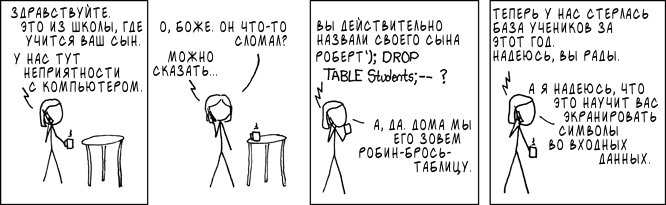
\includegraphics[scale=0.5]{xkcd-327.png}
	\end{center}
\end{frame}

\begin{frame}[fragile]{А как правильно?}
\begin{minted}{python}
with sqlite3.Connection("sql-injection.sqlite3") as db:
  key = input('Text key: ')
  cursor = db.execute("SELECT * FROM Text WHERE owner='user' AND key=?", [key])
  print(list(cursor))
\end{minted}
	Теперь драйвер базы данных знает, что \t{key} "--- это значение от пользователя,
	которое надо \textit{заэкранировать}:
	\begin{center}
		\begin{tabular}{ll}
			Значение: & \t{' OR ''='} \\\hline
			Было:  & \t{... WHERE owner='user' AND key=?} \\\hline
			Стало: & \t{... WHERE owner='user' AND key='\textbackslash' OR  \textbackslash'\textbackslash'=\textbackslash''} \\
		\end{tabular}
	\end{center}
	Независимо от того, какой код мы напишем, SQL-инъекции не случится.

	Мораль: никогда не собирайте SQL-запрос руками из переменных.
\end{frame}

%\section{Запросы посложнее}
\begin{frame}
	\tableofcontents[currentsection]
\end{frame}

\subsection{Группировка строк}

\begin{frame}{GROUP BY}
	\begin{itemize}
		\item Полезно, когда мы хотим посчитать какую-то статистику по подмножествам строк.
		\item Каждая агрегирующая функция начинает работать только внутри группы.
		\item Например, суммарное население стран с разным политическим строем.
		\item Можно группировать по нескольким полям.
		\item Условие \t{WHERE} применяется до группировки.
		\item \t{ORDER BY} применяется после (очевидно, так как группировка от порядка не зависит).
		\item В \t{SELECT} можно использовать только агрегирующие функции и колонки, по которым сделана группировка
			(иначе неясно, из какой строки выбирать).
			Некоторые СУБД ругаются, некоторые делают что-то.
		\item Можно дополнительно отфильтровать результаты после группировки при помощи \t{HAVING}.
	\end{itemize}
\end{frame}

\begin{frame}{Упражнения}
	Посчитайте:
	\begin{enumerate}
		\item Среднюю площадь страны в зависимости от формы правления.
		\item Средний корень площади страны в зависимости от формы правления.
		\item Количество стран с площадью порядка миллиона, порядка двух миллионов, и так далее.
	\end{enumerate}
\end{frame}

%\subsection{Подзапросы}

\begin{frame}{Подзапросы-1}
	\begin{enumerate}
		\item
			\begin{itemize}
				\item Задача: хотим для города найти население страны, в которой он расположен.
				\item В таблице городов есть только код страны, без населения.
				\item Можно сделать подзапрос в условии \t{WHERE}.
			\end{itemize}
		\item
			\begin{itemize}
				\item Задача: хотим найти средний уровень самой грамотной страны по годам.
				\item Надо две агрегатных функции: сначала группируем по годам (чтобы найти победителя), а потом берём среднее.
				\item Можно сделать подзапрос в \t{FROM} (ведь результат SELECT "--- тоже таблица, которую можно назвать).
			\end{itemize}
	\end{enumerate}
\end{frame}

\begin{frame}{Подзапросы-2}
	\begin{itemize}
		\item Задача: хотим вывести информацию по странам плюс население самого большого города.
		\item Эта информация лежит в двух разных таблицах.
		\item SQL позволяет делать \t{SELECT FROM} сразу из нескольких таблиц (получается декартово произведение).
		\item Можно взять декартово произведение городов и стран, оставить только соответствующие, а по оставшимся взять агрегирующую функцию.
		\item Если имена колонок в разных таблицах совпадают, надо явно указывать, к какой мы обращаемся.
		\item Вообще лучше всегда явно указывать, из какой таблицы мы берём колонку, если таблиц несколько.
	\end{itemize}
	Такого сорта выборки происходят очень часто, в реляционной алгебре они зовутся <<соединениями>> (join).
\end{frame}

\subsection{Соединения}

\begin{frame}{Соединения}
	\begin{itemize}
		\item Можно считать синтаксическим сахаром для взятия подмножества декартова произведения.
		\item Лучше отражает суть происходящего и проще читается.
		\item После \t{ON} может быть произвольное условие (это круче, чем в реляционной алгебре).
		\item Обычно там ставят условие <<номер страны в первой таблице равен номеру страны во второй таблице>>.
	\end{itemize}
\end{frame}

\begin{frame}{Ключи и соединения-1}
	\begin{itemize}
		\item Обычно сущностей в базе много и они как-то связны отношениями (<<каждый город лежит ровно в одной стране>>).
		\item Не хочется дублировать информацию в разных таблицах (место занимает, изменять сложно).
		\item Поэтому информация о стране/городе отдельно.
		\item А запрос <<получи объект по вот этому отношению>> возникает.
		\item
			Так как свойства объектов часто меняются, то обычно каждому объекту выдают \textit{первичный ключ},
			по которому его можно опознать.
			Обычно это просто какое-то число (возможно, с автоинкрементом).
	\end{itemize}
\end{frame}

\begin{frame}{Ключи и соединения-2}
	\begin{itemize}
		\item Тогда связи вроде <<в какой стране лежит город>> "--- это просто столбец <<номер страны>> в таблице с городом.
		\item Такой столбец называют \textit{внешним ключом}.
		\item Это даже можно отразить в структуре таблицы (\t{REFERENCES}).
		\item И ещё можно указать, что делать при удалении того объекта, куда мы ссылаемся (\t{ON DELETE CASCADE}).
	\end{itemize}
\end{frame}

\begin{frame}{Упражнения}
	\begin{enumerate}
		\item Вывести для каждой страны максимальный уровень её грамотности за все года.
		\item Вывести для каждой страны номер города-столицы (см. таблицу \t{Capital}).
		\item Вывести для каждой страны название города-столицы (потребуется два \t{JOIN}).
	\end{enumerate}
\end{frame}

\begin{frame}{Соединения, NULL, отсутствие значений}
	\begin{enumerate}
		\item Посчитаем количество стран (239).
		\item Теперь для каждой страны посчитаем количество городов.
		\item Теперь посмотрим, сколько строк получили в результате "--- 232.
	\end{enumerate}
	\begin{itemize}
		\item А всё потому что есть страны, в которых городов нет "--- про них в таблице \t{City} просто нет информации.
		\item И соединение не поможет "--- страна без городов отфильтруется.
		\item Но есть \t{LEFT (OUTER) JOIN} "--- он обязуется добавить в соединение все строчки из <<левой>> таблицы
			(а если не нашлось соответствующих строк, то поля второй в строчке соединения будут \t{NULL}).
		\item С ним надо быть осторожным "--- потому что теперь в строчках соединения могут оказаться \t{NULL},
			которые, скорее всего, не надо учитывать (\t{COUNT(*)}, например, их учтёт).
		\item Ещё бывают аналогичные \t{RIGHT JOIN} и \t{FULL JOIN} (SQLite их не поддерживает).
	\end{itemize}
\end{frame}

\begin{frame}{Классическая шутка}
	\begin{center}
		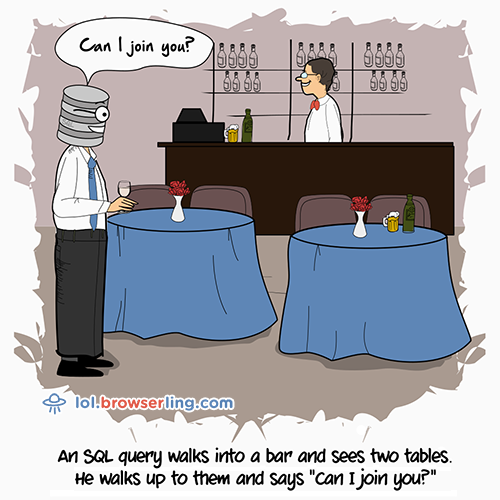
\includegraphics[scale=0.4]{join-two-tables.png}
	\end{center}
\end{frame}

%\subsection{Объединения результатов запросов}

\begin{frame}{UNION}
	\begin{itemize}
		\item Хотим вывести названия всех географических объектов из БД.
		\item Делаем два (или больше) \t{SELECT} с одинаковым количеством столбцов в результате.
		\item Если объединяем их через \t{UNION} "--- то в результате не будет одинаковых строк вообще (даже если они были внутри одного \t{SELECT}).
		\item Если объединяем их через \t{UNION ALL} "--- то просто все результаты объединятся вместе.
	\end{itemize}
	На практике:
	\begin{itemize}
		\item Я ни разу не встречал.
		\item Может потребоваться, если в БД есть похожие таблицы (например, \t{UsersUS} и \t{UsersEU}).
	\end{itemize}
\end{frame}

%\input{03-home}

\end{document}
